\subsection{Data, episode construction and chronological design}
\label{sec:data}
The empirical illustration uses Binance spot BTCUSDT and ETHUSDT one-minute bars for January--August 2026 \citep{binance2026}. Sixteen monthly archives contain 699,840 observations. Before constructing episodes, the download procedure compares each archive with its published checksum and validates the complete minute grid. Checks cover calendar boundaries, microsecond timestamps, duplicates and gaps, close-time consistency, twelve-column structure, finite fields, positive prices, OHLC bounds, nonnegative volumes, integer trade counts and taker-buy volume bounded by total volume. All archives pass. These checks establish consistency of the downloaded bar records; they do not establish that an order could transact at the recorded open.

Each episode represents a hypothetical, normalised sell order completed over fifteen execution opportunities. Let $i$ denote a decision minute, selected at UTC minute offsets $5,35,\ldots,1415$. For total base volume $V_k$ and taker-buy base volume $V_k^B$, the observed signal is
\begin{equation}
 x_i=\frac{\sum_{k=i-5}^{i-1}(2V_k^B-V_k)}{\sum_{k=i-5}^{i-1}V_k},
 \label{eq:imbalance}
\end{equation}
with zero assigned when the denominator vanishes. Only five completed bars enter this signal. The execution-price vector uses opens at minutes $i+1,\ldots,i+15$, leaving a one-minute initial delay after the decision. Relative prices are $p_{ij}=10^4(P_{i+j}/P_i-1)$, where $P_i$ is the decision-minute open. Both the baseline and forecast-dependent schedule use the same denominator and realised prices. There are 48 episodes per asset per day, with nonoverlapping execution horizons. Nonoverlap removes shared execution bars within an asset; it does not imply independence across episodes or assets.

For each asset, a three-month window separates training, calibration and evaluation. The first window trains in January, calibrates in February and evaluates in March; subsequent windows advance by one month, ending with June training, July calibration and August evaluation. The resulting evaluation sample comprises 17,664 episodes across twelve asset--month windows and 184 calendar dates. Each evaluation-month policy uses only the two preceding months. Nevertheless, rolling windows share observations in different roles, and both assets experience common market conditions.

Figure~\ref{fig:rolling} summarises the calendar separation between forecast fitting, exposure fitting and evaluation.
\begin{figure}[htbp]\centering
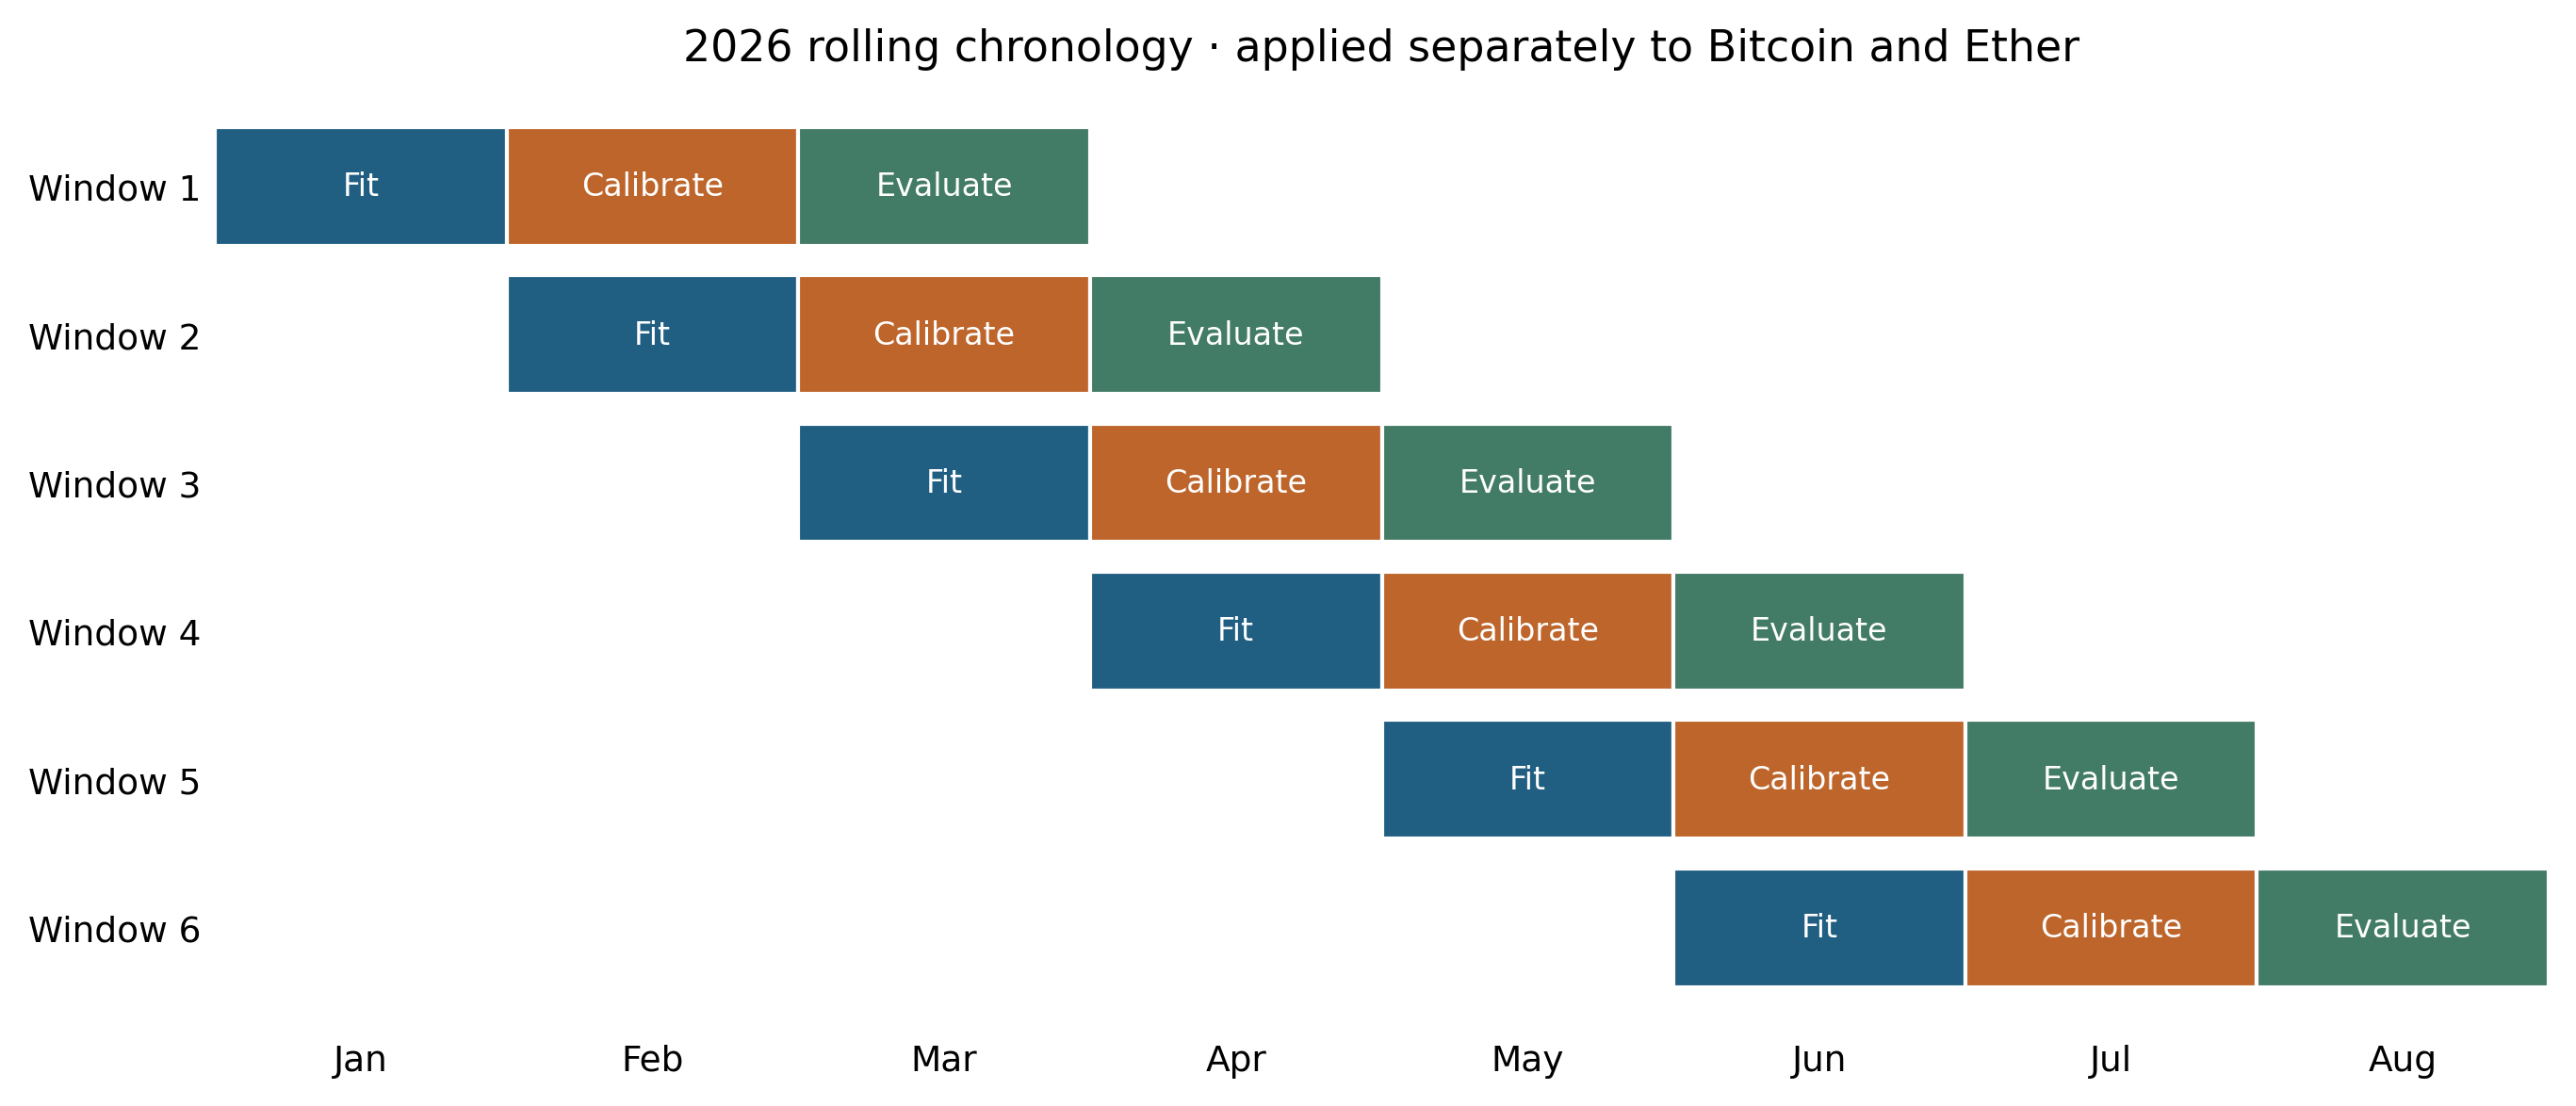
\includegraphics[width=\linewidth]{figures/fig02_rolling_design.png}
\caption{Rolling calendar design for each asset. Each evaluation month follows separate training and calibration months. Calendar ordering prevents within-window look-ahead, but does not make this retrospective extension prospectively preregistered or its entire sample previously unseen.}
\label{fig:rolling}
\end{figure}

The expanded design was recorded after examining an initial Bitcoin evaluation and before computing these expanded outcomes. Bitcoin's August evaluation overlaps that earlier analysis. The study is therefore a retrospective exploratory extension, not an independent confirmation or a prospective preregistration. This chronology motivates reporting every specified window, profile and cost scenario. No additional predictor search, horizon selection or outcome-dependent sample expansion is used in the extension.

\subsection{Forecast construction and matched-endpoint comparisons}
\label{sec:forecastconstruction}
Training fits fifteen ordinary least-squares regressions with intercept, one for each execution horizon. If $\widehat\beta_j$ is the slope on imbalance and $\bar x_{\mathrm{train}}$ its training mean, the forecast is
\begin{equation}
 \mu_{ij}=\widehat\beta_j(x_i-\bar x_{\mathrm{train}}).
\end{equation}
The unconditional fitted intercept is excluded deliberately, so the experiment concerns the estimated imbalance-dependent price profile. The slopes and centring value remain fixed during calibration and evaluation. This simple specification provides an auditable forecast input; it is not selected as the strongest available cryptocurrency predictor.

For each episode, three transformations of the learned profile preserve its final coordinate:
\begin{equation}
 \mu^{\mathrm{parallel}}_{ij}=\mu_{iN},\qquad
 \mu^{\mathrm{ramp}}_{ij}=\frac jN\mu_{iN},\qquad
 \mu^{\mathrm{mirror}}_{ij}=2\mu_{iN}-\mu_{ij},\quad N=15.
 \label{eq:profiles}
\end{equation}
The parallel profile contains no relative-price information across execution opportunities and must recover the no-signal baseline. It is therefore an analytical and numerical control. The ramp imposes a linear path connecting zero to the learned endpoint. The mirror reverses the learned profile's temporal contrasts around that endpoint. These constructions isolate the information discarded by an endpoint summary. In particular, the mirror is a deliberate counterfactual, not a separately estimated forecasting competitor.

Terminal root-mean-square error, directional hit rate and $R^2$ are identical across all four profiles episode by episode. The reported $R^2$ compares squared errors with a zero-return prediction:
\begin{equation}
 R^2_{\mathrm{terminal}}=1-
 \frac{\sum_i(p_{iN}-\mu_{iN})^2}{\sum_i p_{iN}^2}.
\end{equation}
Directional accuracy is the proportion for which forecast and realised terminal signs agree. These quantities remain useful descriptions of endpoint prediction, but they cannot rank the constructed schedules. Holding them fixed is the identification device, rather than a claim that all profiles are equally plausible models of the full price path.

\subsection{Policies, costs and outcome measurement}
\label{sec:policies}
Every profile is passed to the same nonnegative, unit-volume quadratic programme. The baseline minimises the same cost function without a price forecast. The primary specification is $\eta=2$ and $r=1$, with all six combinations of $\eta\in\{0.5,2,5\}$ and $r\in\{0,1\}$ retained as sensitivity checks. The impact parameter imposes a hypothetical monetary charge for concentrated execution. The inventory parameter expresses a preference for reducing remaining inventory; it is not an estimated variance or a realised cash payment. Neither coefficient is fitted to exchange-level fills or depth.

In addition to full exposure to each matched profile, three policies mix the learned schedule with the baseline: a fixed weight of $1/2$, the preceding month's plug-in weight $w_P$, and a lower-percentile weight $w_C$. The plug-in rule maximises mean calibration-month gain on $[0,1]$. For the latter rule, 2,000 resampled calibration days produce aggregate ratios $\overline{(A-B)}/(2\overline C)$; their fifth percentile is clipped to $[0,1]$. Coefficients are aggregated before taking the ratio, rather than averaging unstable episode-level ratios. The code selects zero for negligible aggregate curvature. Each resulting weight is fixed throughout the next evaluation month. The lower-percentile construction is a historical exposure rule, without a prospective coverage or safety guarantee.

The principal outcome is paired objective gain against the baseline, decomposed into price alignment, the baseline-gradient term and curvature cost. Monetary gain is also reported by removing the inventory penalty when scoring the same schedules. Thus it does not substitute a different monetary-optimal policy for the one actually selected. Shifted quantity, $\|u_1-u_0\|_1/2$, describes the fraction of the parent order reallocated between slots. A feasible equality-constrained solution is used when available, with a projected-gradient simplex solver otherwise; the maximum observed KKT residual is $1.29\times10^{-12}$.

\subsection{Aggregation and uncertainty}
\label{sec:uncertainty}
Pooled estimates weight episodes equally, so longer months contribute more observations. Equal asset--month means provide a weighting check. Evaluation intervals use 2,000 bootstrap draws of whole UTC days, retaining both assets together on each sampled date. This grouping preserves within-day serial and cross-asset co-movement. Fitted regressions, calibration weights and policies remain fixed during resampling; calibration and evaluation seeds are recorded in the reproducibility files.

These intervals summarise uncertainty conditional on the selected sample and fitted policies. They neither propagate the complete training and calibration procedure nor accommodate arbitrary dependence across days. No adjustment is made for the multiple profile, window and cost comparisons. Accordingly, interval exclusions of zero are descriptive evidence within the replay, not confirmatory discovery claims. This interpretation also separates uncertainty about the observed paired mean from the unmeasured difference between minute-open proxies and executable fills.
